\chapter{Entorno Hardware}
\label{entornoHW}

En un sistema empotrado el software y hardware están muy vinculados. Para entender el funcionamiento del software de adquisición es muy importante
estar familiarizado con el diseño y funcionalidad del hardware. Impulsados por esta razón en este capítulo procederemos a hacer una descripción de los
aspectos más importantes del hardware que compone el sistema de adquisición. Volvemos a enfatizar que el autor de este trabajo no ha formado parte en
la realización de los módulos hardware que serán descritos a continuación.
\section{BeagleBone Black}
	BeagleBone Black\cite{Beagle}\cite{BeagleWiki} es un computador empotrado, open-source y single board. La placa viene con Linux, distribución
	Angstrom y versión de núcleo 3.8. En la figura \ref{fig:beaglebone} podemos ver un diagrama de bloques que refleja los componentes hardware
	que componen la BeagleBone. A continuación vamos a hacer una breve descripción de los módulos que utilizamos para este trabajo.
	\begin{itemize}
		\item 	ARM CORTEX A8\cite{BeagleCore} y SDRAM. El procesador es suficientemente potente para soportar la distribución Linux y
			satisfacer las necesidades de nuestro software. Los 512MB DDR3 de memoria RAM son suficientes para los propósitos de este
			trabajo.
		\item 	Ethernet Connector. El conector RJ-45 permite establecer una conexión a Internet. Una vez establecida esta conexión los datos
			pueden ser transmitidos al NMDB. También es posible establecer una conexión a la placa vía SSH, de esta manera un operador
			puede realizar operaciones de mantenimiento de forma remota.
		\item	eMMC y microSD. Utilizamos la memoria integrada (eMMC) de 4GB para albergar el sistema operativo y el software de
			adquisición. La microSD es utilizada para guardar los datos y logs producidos por el software de adquisición.
		\item 	Analog Pins. Los 7 pines analógicos permiten usar sensores cuyo output es una señal analógica. Ejemplo de estos sensores son
			las fuentes de alimentación analógicas o los sensores de temperatura, en algunas estaciones la temperatura ambiente se
			monitoriza también. Estos sensores producen señales cuya tensión eléctrica es proporcional al valor de la magnitud medida. 
		\item 	GPIOs. Los \emph{General Purpose Input/Output} permiten trabajar con señales digitales, tanto de entrada como de salida. Un
			ejemplo de uso es la señal de Reset de la FPGA, señal digital activa a bajo nivel.
		\item	UARTs. La placa ofrece 4 puertos serie de los que utilizamos 2 para comunicarnos con la FPGA.
	\end{itemize}
	\begin{figure}[h]
		\centering
		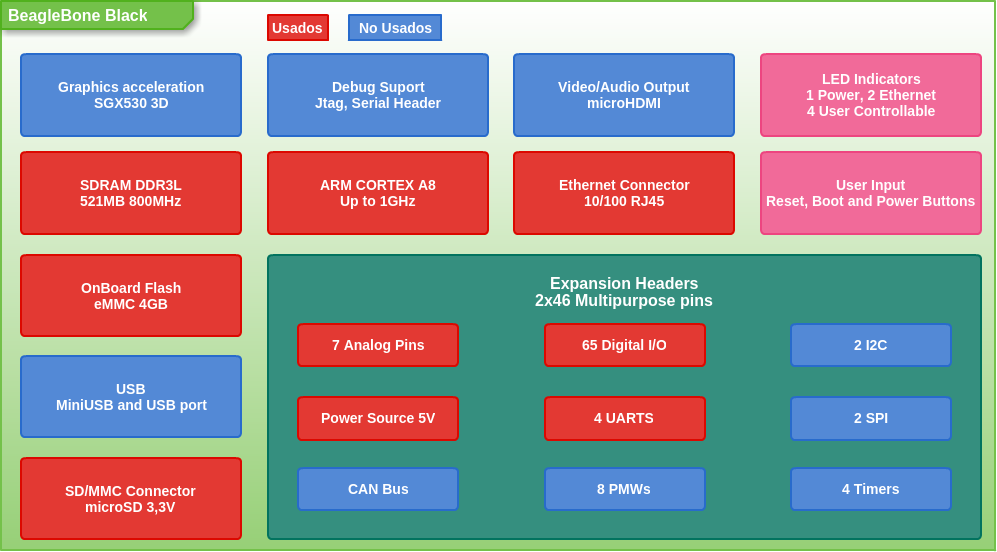
\includegraphics[keepaspectratio, width=1\textwidth]{./img/beaglebone.png}
		\caption{BeagleBone Black. Diagrama de bloques hardware}
		\label{fig:beaglebone}
	\end{figure}
	\par
	Fijándonos en la figura \ref{fig:beaglebone} podemos ver que muchos de los módulos son accesibles mediante los conectores de
	expansión\cite{BeagleWikiExp}. Estos conectores tienen 2x46 pines, de los cuales muchos son multipropósito. Estos pueden ser configurados para tener
	funcionalidades diversas y además esta configuración puede ser realizada de forma dinámica. La configuración de los pines se realiza mediante
	el \emph{Device Tree Overlay}, estructura de datos que se utiliza para describir el hardware. En la realización de este trabajo no lidiamos
	con este mecanismo, sino que utilizamos una librería que facilita el trabajo. La librería utilizada es \emph{Adafruit BeagleBone IO
	Python}\cite{AdaFruitGit}. Esta ayuda a configurar dinámicamente los pines de expansión, además ofrece métodos para
	operar sobre estos una vez configurados.

\section{FPGA}
	La FPGA es el núcleo fundamental del sistema, ya que, se encarga de procesar las señales y transmitir la información al software de
	adquisición. Una FPGA es un circuito integrado, que está formado por unidades lógicas cuya interconexión y funcionalidad pueden ser
	configurados. Esta configuración está definida por el \emph{IP core} integrado, por lo tanto, es este el que establece la funcionalidad de una
	FPGA. En esta sección vamos a hacer una descripción funcional de la FPGA, por consiguiente será explicado el \emph{IP core} de esta.  En la
	figura \ref{fig:fpga} podemos ver un diagrama de bloques que refleja los módulos funcionales y interfaces que el este posee.
	\begin{figure}[h]
		\centering
		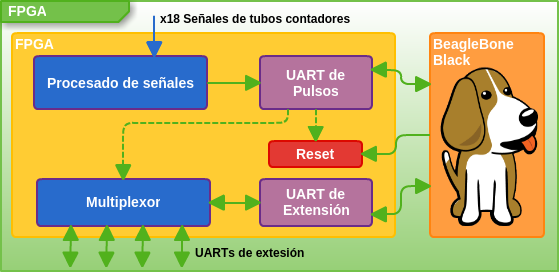
\includegraphics[keepaspectratio, width=1\textwidth]{./img/fpga.png}
		\caption{FPGA. Diagrama de bloques.}
		\label{fig:fpga}
	\end{figure}	
	\subsection{Procesado de pulsos}
		Como hemos comentado la FPGA es la encargada de procesar las señales y trasmitir la información a la BeagleBone Black. Esta transmisión
		se realiza mediante una línea serie asíncrona de 1Mbps. La línea está controlada por una UART(Universal Asynchronous
		Receiver-Transmitter) a la que nos referiremos como \emph{UART de pulsos}. En las tablas \ref{tab:FPGAUartPulso},
		\ref{tab:FPGAUartOver} y \ref{tab:FPGAUartCont} podemos ver el formato de los datos transmitidos. Vemos que hay tres mensajes
		diferentes que la FPGA puede transmitir.
		\begin{itemize}
			\item	En la tabla \ref{tab:FPGAUartPulso} podemos ver el formato del primer mensaje que vamos a discutir. Este mensaje se
				compone de tres bytes que dan información sobre el ancho de un pulso. El mensaje permite identificar el canal en el
				que se ha producido el pulso, el nivel (alto/bajo) y la longitud de este. Los pulsos de nivel alto representan la
				detección de una partícula por los tubos contadores y el ancho del pulso es proporcional a la energía de la partícula
				detectada. La longitud de los pulsos de nivel bajo también se mide para poder identificar pulsos con pequeña
				separación temporal, que podrían indicar la presencia de un fenómeno físico denominado multiplicidad.
			\item 	En la siguiente tabla \ref{tab:FPGAUartOver} podemos apreciar el mensaje de estado que la FPGA genera. Dado que la UART usa
				una FIFO de tamaño fijo es posible que la esta se llene y se pierdan mensajes. En este caso la FPGA genera un mensaje
				de estado que es transmitido para indicarle al software que se han producido perdidas de datos.
			\item	Además de medir el ancho de los pulsos la FPGA lleva la cuenta de pulsos recibidos para cada canal. Esta información
				puede ser solicitada por la BeagleBone Black utilizando el comando apropiado(ver tabla \ref{tab:FPGAUartComm}). En la
				tabla \ref{tab:FPGAUartCont} podemos ver el formato en el que se transmite la información de las cuentas. Los bytes 2,
				3 y 4 son transmitidos 18 veces, una vez para cada canal. Después de transmitir la información de las cuentas la FPGA
				reinicia los contadores para cada canal.
		\end{itemize}
		En la figura \ref{fig:fpgaWave} podemos observar un ejemplo de la secuencia de datos transmitidos por la \emph{UART de pulsos}, junto a
		estos podemos apreciar los estímulos que los causan. 

		\begin{table}[h]
			\tiny
			\begin{tabularx}{\textwidth}{|l|c|c|X|c|c|c|c|c|}
				\hline
				\rowcolor[HTML]{C0C0C0} 
				\multicolumn{1}{|r|}{\textbf{Bit}}    	& 7 & 6          & 5 				& 4 	       & 3 	     & 2 	  & 1          & 0 	     \\ \hline
				\cellcolor[HTML]{C0C0C0}\textbf{Byte 1} & 0 & 1          & 0  				& \multicolumn{5}{c|}{Canal (0-17)}				     \\ \hline
				\cellcolor[HTML]{C0C0C0}\textbf{Byte 2} & 1 & Dato (6)	 & Dato (5)      		& Dato (4)     & Dato (3)    & Dato (2)   & Dato (1)   & Dato (0)    \\ \hline
				\cellcolor[HTML]{C0C0C0}\textbf{Byte 3} & 1 & X          & Nivel ('1'->alto, '0'->bajo) & Dato (11)    & Dato (10)   & Dato (9)   & Dato (8)   & Dato (7)    \\ \hline
			\end{tabularx}
			\caption{\emph{UART de pulsos}. Palabra de ancho de pulso}
			\label{tab:FPGAUartPulso}
			\begin{tabularx}{\textwidth}{|l|c|X|X|X|X|X|X|X|}
				\hline
				\rowcolor[HTML]{C0C0C0} 
				\multicolumn{1}{|r|}{\textbf{Bit}} 	& 7 & 6 		       & 5 		       & 4		       & 3 		       & 2		       & 1          	       & 0			\\ \hline
				\cellcolor[HTML]{C0C0C0}\textbf{Byte 1} & 0 & 0                        & OverFlow FIFO Tubo 5  & OverFlow FIFO Tubo 4  & OverFlow FIFO Tubo 3  & OverFlow FIFO Tubo 2  & OverFlow FIFO Tubo 1  & OverFlow FIFO Tubo 0	\\ \hline
				\cellcolor[HTML]{C0C0C0}\textbf{Byte 2} & 1 & OverFlow FIFO Tubo 12    & OverFlow FIFO Tubo 11 & OverFlow FIFO Tubo 10 & OverFlow FIFO Tubo 9  & OverFlow FIFO Tubo 8  & OverFlow FIFO Tubo 7  & OverFlow FIFO Tubo 6	\\ \hline
				\cellcolor[HTML]{C0C0C0}\textbf{Byte 3} & 1 & Almost Full FIFO General & OverFlow FIFO General & OverFlow FIFO Tubo 17 & OverFlow FIFO Tubo 16 & OverFlow FIFO Tubo 15 & OverFlow FIFO Tubo 14 & OverFlow FIFO Tubo 13	\\ \hline
			\end{tabularx}
			\caption{\emph{UART de pulsos}. Palabra de estado}
			\label{tab:FPGAUartOver}
			\begin{tabularx}{\textwidth}{|l|X|c|c|c|c|c|c|c|}
				\hline
				\rowcolor[HTML]{C0C0C0} 
				\multicolumn{1}{|r|}{\textbf{Bit}}    	 & 7 & 6           & 5 		& 4 	      & 3 	    & 2 	 & 1           & 0 	     	\\ \hline
				\cellcolor[HTML]{C0C0C0}\textbf{Byte 1}  & 0 & 1           & 1  	& X	      & X	    & X	  	 & X	       & X	     	\\ \hline
				\cellcolor[HTML]{C0C0C0}\textbf{Byte 2}  & 1 & Dato0 (6)   & Dato0 (5) 	& Dato0 (4)   & Dato0 (3)   & Dato0 (2)  & Dato0 (1)   & Dato0 (0)  	\\ \hline
				\cellcolor[HTML]{C0C0C0}\textbf{Byte 3}  & 1 & Dato0 (13)  & Dato0 (12)	& Dato0 (11)  & Dato0 (10)  & Dato0 (9)  & Dato0 (8)   & Dato0 (7)  	\\ \hline
				\cellcolor[HTML]{C0C0C0}\textbf{Byte 4}  & 1 & X	   & X	 	& X	      & X	    & X		 & Dato0 (15)  & Dato0 (14)	\\ \hline
				\cellcolor[HTML]{C0C0C0}\textbf{Byte 5}  & 1 & Dato1 (6)   & Dato1 (5) 	& Dato1 (4)   & Dato1 (3)   & Dato1 (2)  & Dato1 (1)   & Dato1 (0)  	\\ \hline
				\cellcolor[HTML]{C0C0C0}\textbf{......}  & . & .........   & ......... 	& .........   & .........   & .........  & .........   & .........  	\\ \hline
				\cellcolor[HTML]{C0C0C0}\textbf{Byte 55} & 1 & X	   & X	 	& X	      & X	    & X		 & Dato17 (15) & Dato17 (14)	\\ \hline
			\end{tabularx}
			\caption{\emph{UART de pulsos}. Palabra de cuentas}
			\label{tab:FPGAUartCont}
			\begin{tabularx}{\hsize}{|c|X|}
		  		\hline
				\rowcolor[HTML]{C0C0C0} 
		  		Commando & Descripción                            \\\hline
		  		0x00     & Configura multiplexor para aparato 1   \\\hline
		  		0x01     & Configura multiplexor para aparato 2   \\\hline
		  		0x02     & Configura multiplexor para aparato 3   \\\hline
		  		0x03     & Configura multiplexor para aparato 4   \\\hline
		  		0x10     & Reset general del sistema              \\\hline
		  		0x11     & Solicita la transmisión de las cuentas \\\hline
			\end{tabularx}
			\caption{\emph{UART de pulsos}. Commandos}
			\label{tab:FPGAUartComm}
		\end{table}
		\begin{figure}[h]
			\centering
			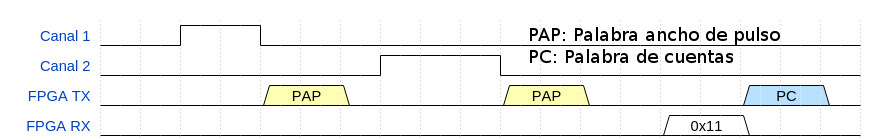
\includegraphics[keepaspectratio, width=1\textwidth]{./img/fpgawave.png}
			\caption{FPGA. Diagrama de eventos.}
			\label{fig:fpgaWave}
		\end{figure}
	\subsection{Multiplexor}
		Tal y como explicamos en el capítulo de introducción, el sistema de adquisición debe monitorizar la presión atmosférica, el
		funcionamiento de las fuentes de tensión y en muchos casos la temperatura ambiente. Al igual que muchos otros dispositivos que pueden
		ser necesarios, la mayoría de estos sensores hacen uso de un puerto serie. Estos son manejados según el patron \emph{Master-Slave} y
		generalmente intercambian poca información, por consiguiente, pueden compartir un puerto serie. El mecanismo que resuelve este
		problema está implmentado en el \emph{IP core}. Este consiste en una UART a la que nos referiremos como \emph{UART de extensión}. Esta
		está conectada a un multiplexor, que es el encargado de realizar la conmutación entre los cuatro dispositivos soportados. El estado
		del multiplexor puede cambiarse enviando comandos por la \emph{UART de pulsos}, de acuerdo a la especificación presentada en la tabla
		\ref{tab:FPGAUartComm}. Ejemplo de dispositivos que requiren un puerto serie son el barómetro \emph{BM35} utilizado en CALMA, varias
		fuentes de alimentación comerciales, estaciones meteorológicas, GPS, etc.
	\subsection{Reset}
		El \emph{IP core} permite realizar un Reset del estado interno de la FPGA. Todas las variables son puestas a sus valores iniciales,
		excepto el multiplexor que mantiene su estado. Para la realización de dicho Reset son exportadas tres interfaces. La primera es un
		boton hardware accesible de forma física. La segunda es un commando trasmitido por la \emph{UART de pulsos}, de acuerdo a la
		especificación presentada en la tabla \ref{tab:FPGAUartComm}. Finalmente, la tercera es una señal digital activa a bajo nivel. Dicha
		señal definida como \emph{BS1}, está conectada al pin \emph{P9\_42(GPIO\_7)} de la BeagleBone Black, por consiguiente, es accesible
		desde nuestro software de adquisición.
